\subsubsection{Description/circuitry}
% Describe the concept and circuitry of the latching/reset system for a tripped IMD or AMS.  Describe the method for resetting the IMD and AMS.

\subsubsection{Wiring/cables/connectors}
\iffalse Describe wiring, show schematics, describe connectors and cables used and show useful data regarding the wiring.  If not detailed in section 2.1, be sure to show how the device opens the shutdown circuit.\fi
% SDC monitoring scheme 
Measuring, what was original problem, is done by two optocouplers in \gls{ecub}. \ref{fig:SDC-schematic}- Example of used \gls{sdc} monitoring with optocouplers.
\subsubsection{Position in car}
%Provide CAD-renderings showing the relevant parts. Mark the parts in the rendering, if necessary.
Latch as well as reset of \gls{imd} and \gls{bms} error is placed in \gls{ecub}box on the back of car. See \ref{fig:ecub_position}.

\begin{figure}[H]
	\centering
	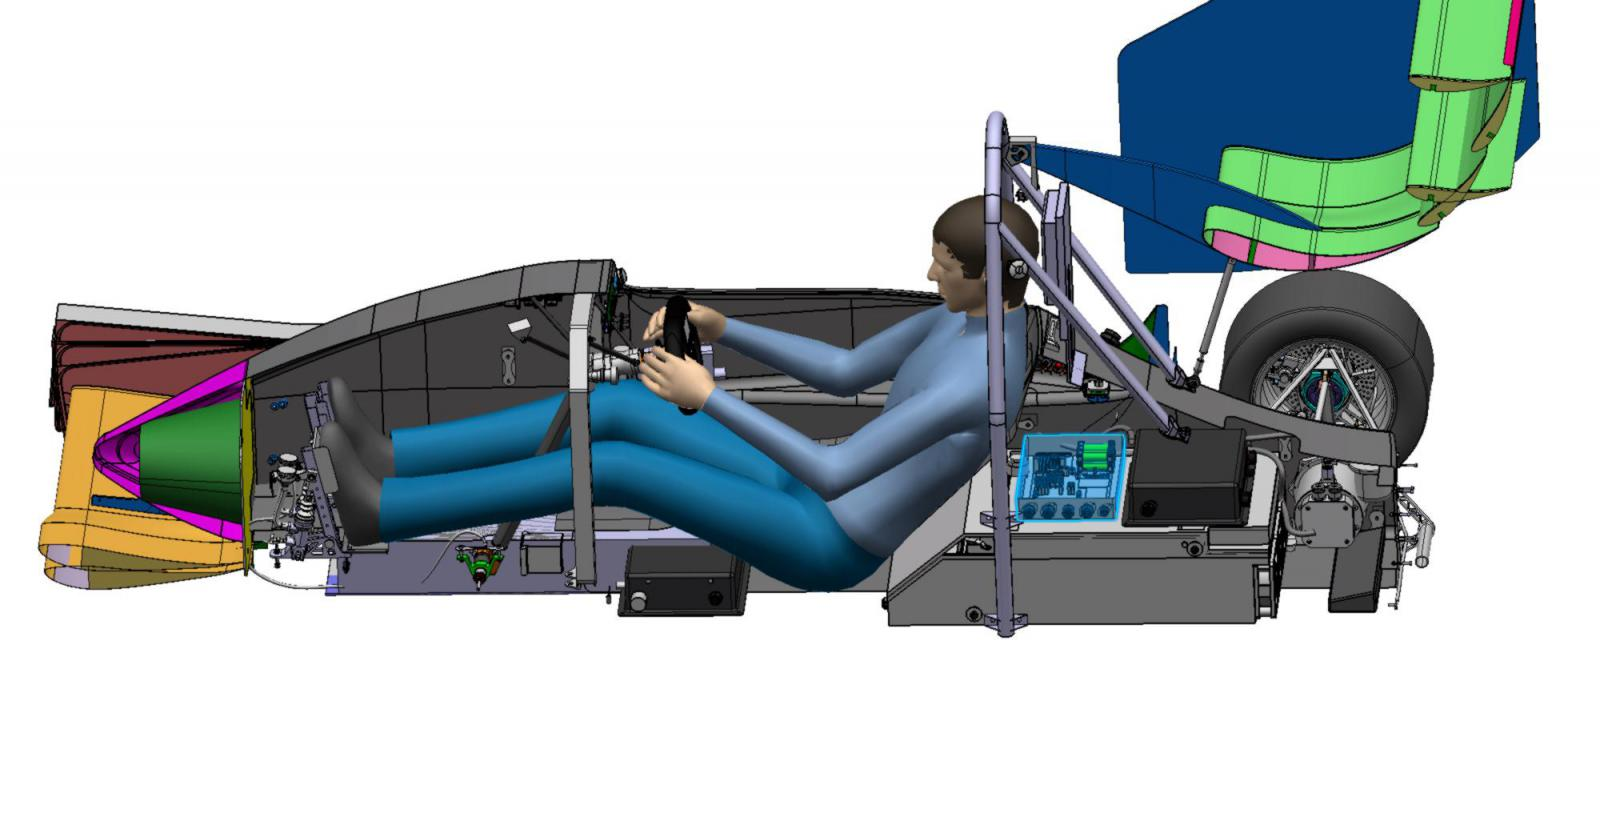
\includegraphics[width=\textwidth]{./img/ECUB_POSITION.png}
	\caption{\gls{bspd} schematic sheet}
	\label{fig:ecub_position}
\end{figure}